\documentclass[11pt]{article}
\usepackage{fullpage}
\usepackage[margin=2.5cm, bottom=3cm]{geometry}
\usepackage{amsmath,amsthm,amsfonts,amssymb,amscd}
\usepackage{mathrsfs}
\usepackage{fancyhdr}
\usepackage{hyperref}
\usepackage{graphicx}

\hypersetup{
colorlinks=true,
linkcolor=blue,
linkbordercolor={0 0 1}
}
\linespread{1.25}
\pagestyle{fancyplain}
\headsep 1.5em
\headheight 14pt

\title{Infant Cry Prediction}

\author{Jake Callahan, Taylor Paskett}

\begin{document}
\maketitle

\begin{abstract}
   The problem of identifying why an infant is crying is one that has plagued parents since the dawn of time.
   There is sparse research to suggest that infants do not modify their cries based on the reason for their crying, but we propose that it might be possible to use machine learning techniques to identify the reasons for an infant's cry. 
   In this paper we explore several techniques to classify infant cries, including classical machine learning techniques and more modern deep learning methods, and ultimately conclude that there is compelling evidence to suggest it is possible for a machine learning model to classify the reasons for infant cries with a high degree of accuracy.
\end{abstract}

\section{Problem Statement and Motivation}
Parents of newborns are constantly exposed to the cries of their child.
After some time, parents can often recognize the cries of their newborn and what they mean [citation here].
For instance, a parent may be able to differentiate between a "hungry cry" and a "tired cry".
This is an acquired skill, however, and incessant crying has been shown to have adverse effects on parents.
Zeifman et al. have suggested that there are "physiological and neural responses to crying that may predispose some adults to maltreat infants." [\url{https://www.ncbi.nlm.nih.gov/pmc/articles/PMC5494986/#R5}]
Most people agree that mistreating infants is despicable.
However, instead of just agreeing, it might be helpful for parents to actually have tools at their disposal so that they can more calmly, rationally deal with a crying baby.

Some research suggests that an infant's cries may not differentiate between causes, only indicating the severity of the infant's distress.
This research posits that parents need other contextual clues to properly determine the cause of crying.
However, it is unclear what methods the authors used to differentiate cries.
We believe that it may be possible for a computer to classify crying by sound alone.
If this is possible, it could assist parents, helping them diagnose the source of their child's cries.
For good parents who would never have abused their children, this could be a source of direction and sanity for them.
In less desirable parenting situations, being able to classify cries could help reduce maltreatment of infants.

In our project, we hope to address both of the following questions:
\begin{enumerate}
   \item Do different "cry types" exist? Meaning, are there objective differences between an infant's cries based on what they want?
   \item If cry types exist, can we accurately predict these cry types using audio of the infant?
\end{enumerate}

This problem has been studied by others, such as [the people we got our data from].
They found that [INSERT FINDINGS HERE].


\section{Data}
The data we use for this analysis is sourced from a corpus entitled
the "Donate-a-Cry Corpus" [https://github.com/gveres/donateacry-corpus].
This corpus, a compilation of audio recordings of babies crying, appears to have originally been collected as part of a campaign entitled the "Donate-a-Cry Campaign" in Sweden in 2015.
More infomation about this campaign cannot be ascertained as the listed campaign website in the github repository has been converted into a website for Japanese escorts.
Further work on this dataset, including removing background noise, standardizing sample rates, and eliminating outliers, was completed by researchers at the Royal Institute of Technology of Sweden in 2018.

This dataset contains 457 recordings (all in .wav format and all about 7 seconds long) of babies crying, each a different baby and each collected by the baby's mother.
These recordings were each labeled with an assumed reason for the cry instance by the mother and then submitted to the corpus.
The data contain 5 different label categories: belly pain, needing to burp, hunger, tiredness, and discomfort.

The two main issues to deal with in working with this cry corpus have to do with label representation.
Over 350 of the audio files belong to the "hungry" category, comprising over $2/3$ of the dataset, while none of the other four categories contained more than 26 audio files.
To combat this, we first cut each audio file down to 3 seconds in length under the assumption that any information contained in the first half of a cry would also be contained in the second half.
We discarded the second halves of all of the hungry crying data, and kept the second halves of all other categories.
This allowed us to effectively double the number of samples we had in each category.
Second, we duplicated each non-hungry datapoint and added small amounts of noise proportional to each wavelength of the sample.
This allowed us to create even more unique data corresponding to these labels while feeling safe that these new datapoints would contain the same features that the non-synthetic data contained.
This process left us with exactly 400 unique datapoints to use in training and testing our models.

To extract features from this data, we took the Fourier transform of each sound file, normalizing the frequencies produced.
This allowed us to eliminate the time dimension and analyze if the frequencies in a baby's cry contain the requisite information to differentiate the reasons for crying.


\section{Methods}
\subsection{Baseline Methods}
We began our analysis by testing the performance of several models to see how well a variety of models handled our dataset.
In doing so, we found a performance baseline to surpass.
In further iterations, we used models with more intentional choices of hyperparameters, architectures, etc.
The following table outlines the models we used initially and their accuracies on both the raw audio data as well as the frequency data, obtained via Fourier transform.
Note that since there are five classes, a score of $20\%$ is about what we would expect if we randomly guessed.
\begin{center}
   \begin{tabular}{| r | c | c |}
      \hline
      \textbf{Method} & \textbf{Raw Audio Score} & \textbf{Frequency Score}  \\
      \hline
      Ordinary Least Squares & 0.15 & 0.23 \\
      Gaussian Discriminant Analysis & 0.40 & 0.38 \\
      Linear Discriminant Analysis & 0.66 & 0.49 \\
      Support Vector Machine & 0.71 &  0.68\\
      XGBoost & 0.76 & 0.68 \\
      Random Forest Classifier & 0.74 & 0.5\\
      \hline
   \end{tabular}
\end{center}
As we can see, in almost every case, the raw audio data performed better than the frequency data.
This was surprising to us, but it indicated that the Fourier transform may be removing useful features from the data.
One explanation for this is could be that in the three-second timeframe, the babies' cries we analyze are not very periodic, so the Fourier transform is not very useful.
Recall that the Fourier transform decomposes a signal into constituent frequencies.
A baby's cry does not sound like a single note from a piano; the cry is composed of a cacophony of superimposed frequencies, which vary over time.
By taking the Fourier transform of the entire three seconds of crying, we may not be extracting very useful features because we're effectively taking the average frequencies over the entire three seconds.
This might lose the information that allows us to differentiate their cries.
This hypothesis has some evidence based on the sample variances of the training data.
Using the 2-norm to measure distance from the mean, the frequency training data has a variance of about $ 300 $, while the raw audio data has a variance of about $ 1.1 \times 10^{14} $.

In the following sections, we attempted to perform better than Linear Discriminant Analysis (LDA), the XGBoost classifier, and the Random Forest classifier.
We were able to outperform these methods when we used neural networks, as will be seen later.

\subsection{Principle Component Analysis}
Surprisingly, running a PCA on both the frequencies gathered from the Fourier transform and on the raw wavelength data, we found that much (TODO: how much exactly?) of the variance could be explained with just the first 25\% of components.

TODO: Put PCA graph here.

\subsection{Mel-Frequency Cepstral Coefficients}
In automatic speech recognition, Mel-frequency Cepstral Coefficients (MFCCs) have been a popular feature to use, especially in tandem with Gaussian Mixture Hidden Markov Models (GMMHMMs).
We wanted to try using a GMMHMM on our baby cry dataset because these models have been successful in classifying speech in the past.
In addition to being combined with GMMHMMs, MFCCs have several advantages compared to Fourier transform frequencies, which we will outline in this section.
First, we review how the MFCCs are computed.
MFCCs are computed from audio data using the following steps:
\begin{enumerate}
   \item divide the audio into frames;
   \item apply a window function to each frame;
   \item compute the power spectrum of each windowed frame;
   \item apply a Mel-scaled filter bank;
   \item decorrelate the values from step 4 by taking the discrete cosine transform (DCT).
\end{enumerate}

The first step, framing, solves the problem we mentioned above concerning the Fourier transform.
It does not make sense to find the frequencies of an entire baby's cry because we lose the change in frequencies over time.
Framing divides the audio signal into a number of frames (in our case, 49).
These frames may have overlap; a pretty typical frame overlap is about 50\%.
After framing, we can compute the frequencies of each frame and our model will be able to observe and learn from the frequencies changing in time.

In the second step, we apply a window to each frame.
A common window function is the Hamming window: \begin{align*}
    w[n] &= a - (1 - a) \cos \left ( \frac{2 \pi n}{N} \right).
\end{align*}
The constant $ a $ is chosen so the window only takes on values between $ [0, 1] $.
Dividing by $ N $ (the number of samples in each frame) in the cosine term makes it so the peak of the curve occurs in the middle of the frame.
This step is calculated by multiplying the $ n $th wavelength value of each frame with $ w[n] $.
This has the effect of tapering the wavelengths; even though there's overlap between frames, the values at the edge of each frame will be tapered so that we do not overemphasize these values.

The third step computes the power spectrum of each windowed frame, which is just a scaled version of the Fourier transform.
Specifically, the power is given by \begin{align*}
    P(x) = \frac{|\mathscr{F}(x)|^2}{N},
\end{align*}
where $ \mathscr{F} $ denotes the discrete Fourier transform and $ N $ is the number of samples in $ x $.

In step four, we apply a Mel scale to the frequencies computed in the last step.
The Mel scale relates frequencies to human hearing.
At low frequencies, humans are able to discern very small changes.
However, at higher frequencies, humans lose the ability to perceive such granularity.
The Mel scale filters the frequencies so that we now have a more dense set of lower frequencies and a sparser set of high frequencies, modeling human hearing.

Finally, because the Mel-scale frequencies are highly correlated in step four, a DCT is applied to them in order to decorrelate them.
Decorrelating them means that in a Hidden Markov Model (HMM) classifier, diagonal covariance matrices can be used to model the features, which is advantageous numerically.

\subsection{Gaussian Mixture Hidden Markov Model}
After computing the MFCCs, we used a GMMHMM classifier to predict each baby's cry type.
This model was slow to train, and sadly, even after a hyperparameter grid search, its score was only $ 0.44 $.
So, both LDA, XGBoost, and the Random Forest classifier outperformed GMMHMM.
At this point, it seemed very likely that our best option would be neural networks:
even though GMMHMM classifiers were often used for automatic speech recognition in the past, neural networks have since replaced them as the industry standard.

\subsection{Neural Networks}
Neural networks have become widely accepted as the best method for performing speech recognition, we wish to apply them to our problem but one of the of the main problems with using neural networks on our dataset is our lack of data:
with only 400 data points, we strongly risk overfitting.
Similarly, if we use the raw audio data to train a neural network, there is a chance that the resulting model will not be generalizable when new data is used.
In order to solve both of these problems, we used Mel Spectrograms as the input data to our networks.
Mel spectrograms are computed in the same exact way as MFCCs except for the final decorrelation step, which is omitted. 
Since neural networks perform well with correlated data, this shouldn't be a problem.
We believe there to be two ways in which using Mel spectrograms can improve performance in our classification task. First, it  will help the models to be more generalizable in two ways:
\begin{itemize}
   \item Spectrograms can conveniently be thought of as images, which allows for the use of convolutional neural networks and provides an easy way to further augment our data by translating and skewing the spectrograms.
   \item The spectrograms may be more robust in terms of being similar to new data we might wish to classify.
\end{itemize}
Second, Mel Spectrograms correlate frequency with time, which can possibly provide valuable information to a classifier such as an LSTM or CNN.
\begin{figure}[!htb]
\begin{center}
   \includegraphics[width=0.4\linewidth]{../rnn_models/example_mels.pdf}
   \caption{An example Mel spectrogram of a baby cry with the label "hungry"}
\end{center}
\end{figure}
\subsubsection{Recurrent Neural Network}
\begin{figure}[!htb]
\begin{center}
   \includegraphics[width=0.8\linewidth]{../rnn_models/rnn_loss_acc.pdf}
   \caption{RNN loss and accuracy using a batch size of 16 over 100 epochs}
\end{center}
\end{figure}
Recurrent neural networks are a commonly used tool in the field of audio classification. 
They perform remarkably well on tasks that require some form of time-dependent learning, and since our classification task involves an element of time dependency, we thought it prudent to begin with a recurrent neural network.
We chose to implement a simplified version of the Bidirectional Long-Short Term Memory Network proposed by Keren and Schuller [TODO: citation] using code provided by Carlo Lepelaars [https://www.kaggle.com/carlolepelaars/bidirectional-lstm-for-audio-labeling-with-keras]. This is a special form of recurrent neural network that can capture time-dependent information independent of ordering; that is, it can capture future and past information in each time step.
This network was designed for usage with time-related image inputs, making it a seemingly suitable choice for our classification task. 
We structured our network with a single bidirectional LSTM layer (a layer containing one forward LSTM layer and one backward LSTM layer) followed by an attention pass and small dropout (0.2). We then pass to a dense layer with exponential linear unit activation, another dropout, and a final 5-node dense layer activated with softmax.
Using this model we achieved 70\% validation accuracy and 90\% training accuracy (See: Figure 2). 
While encouraging, it is possible this model is overfitting to the data provided.


\subsubsection{Convolutional Neural Network}
Our convolutional neural network had the following architecture.
It contained four main sections, with the first three having the same design: a convolutional layer, a relu activation, and a max pooling layer.
The fourth section flattens the data, uses a relu activation, then adds an aggressive dropout of $50 \%$.
Finally, the output layer consists of five nodes with a softmax activation. We achieved validation accuracy above 80\% using only Mel spectrograms generated from our original audio files and without performing any augmenting processes on the image data.
\begin{figure}[!htb]
\begin{center}
   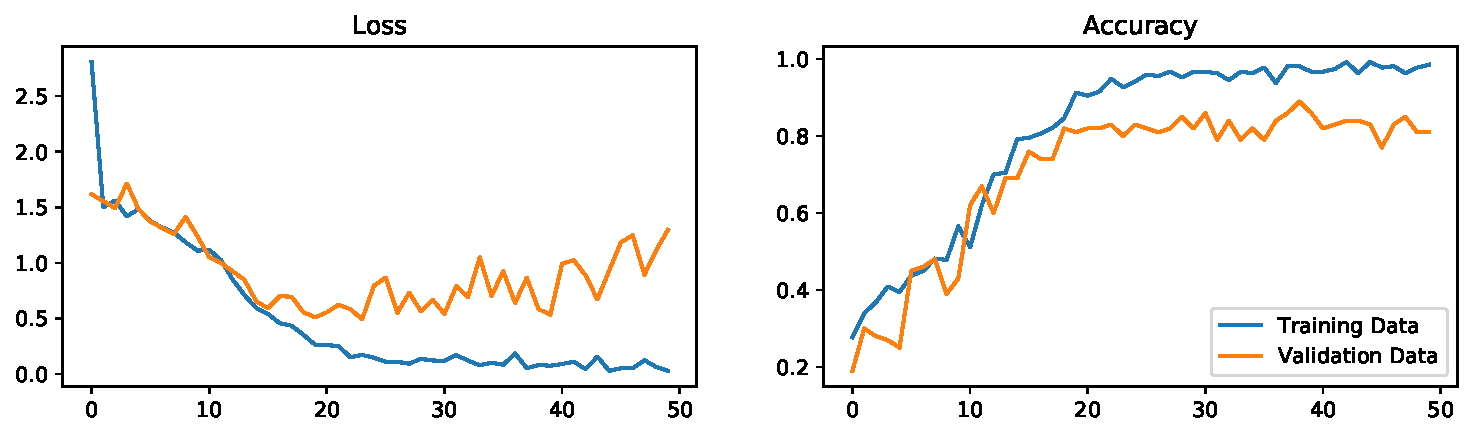
\includegraphics[width=0.8\linewidth]{../cnn_models/first_try_loss_acc.pdf}
   \caption{CNN loss and accuracy using a batch size of 16 [TODO: confirm batchsize] over 50 epochs}
\end{center}
\end{figure}

\section{Results}
At this point, we have successfully identified a featureset / model / hyperparameter combination that performs our classification task better than $\sim70\%$ average accuracy.
The baseline models with most consistent performance were the Random Forest classifier and the LDA algorithm.
The baseline models that performed the worst were the GDA algorithm and the OLS algorithm.
Once we used Neural Networks, we were able to achieve higher than $ 80 \% $ accuracy, which is quite good. In particular, the CNN architecture performed noticeably better than 


\section{Analysis}
First, it appears that there was important information to be captured in the time domain as evidenced by the poor performance of the Fourier-trained models., However, the superior performance of the CNN suggests that it was not the sequential information that mattered. 
Thus, it appears that Mel spectrogram image data contained sufficient information to teach a model to recognize cry types.
Overall, as our models (especially the neural networks) were able to achieve high accuracy, we feel there is evidence to suggest that there are machine-discernible patterns differentiating cry types.
Although these results are encouraging, they are limited in scope at this time.  
The first step in expanding this scope would be to obtain more data and see if the models still perform similarly. 
Further, setting up a formalized experiment in which we have control over the data collection process could yield even more fruitful results.

\section{Ethical Implications}
As with all machine learning applications, there are drawbacks to relying on computer-based decision making. 
To a parent trying to care for an infant, a misclassification might lead to more stress for both parent and child, and, in situations where abuse is already a possibility, exacerbate the problem due to increased frustration. 
Further, when discussing machine-assisted parenting, we must consider the consequences of outsourcing parental intuition: could a cry classifier damage or inhibit the parent-child relationship developed in infancy? 
We believe that a tool like the one we propose would be a net benefit to parents and children, but the risks must still be analyzed.
\section{Conclusion}
We believe the results we have found to be encouraging but ultimately inconclusive. Formalized testing, a more robust data set, and more data augmentation would provide much more insight into whether a machine learning cry detection tool would be useful in assisting parents in quieting their little ones. 
\end{document}
